
\documentclass{beamer}
\usepackage{ragged2e}
\usepackage{CJKutf8}
\usepackage{tikz}
\setbeamertemplate{theorems}[numbered]
\justifying\let\raggedright\justifying
\begin{document}
\begin{CJK*}{UTF8}{gbsn}


  
\theoremstyle{definition}
\newtheorem{Def}{定义}
\theoremstyle{example}
\newtheorem*{Ex}{例:}
\newtheorem*{Exercise}{习题}

\date{}
\author{陈建文}
\title{习题讲解}
\begin{frame}
  \titlepage
\end{frame}

\begin{frame}
\begin{Exercise}
  下列命题中哪个是真的?

A. 对任意集合$A$,$B$,$2^{A\cup B} = 2^A \cup 2^B$。

B. 对任意集合$A$,$B$,$2^{A\cap B} = 2^A \cap 2^B$。

C. 对任意集合$A$,$B$,$2^{A\setminus B} = 2^A \setminus 2^B$。

D. 对任意集合$A$,$B$,$2^{A\bigtriangleup B} = 2^A \bigtriangleup 2^B$。

\end{Exercise}
\pause
  \begin{Def}
  集合$S$的所有子集构成的集合称为$S$的幂集,记为$2^S$或者$\mathcal{P}(S)$。
\end{Def}
  \begin{Ex}
    \begin{itemize}
    \item $2^\phi=\{\phi\}$
    \item $2^{\{\phi\}}=\{\phi,\{\phi\}\}$
    \item $2^{\{\phi,\{\phi\}\}}=\{\phi,\{\phi\},\{\{\phi\}\},\{\phi,\{\phi\}\}\}$
    \end{itemize}
    \end{Ex}
  \end{frame}

  
\begin{frame}
\begin{Exercise}
  下列命题中哪个是真的?

A. 对任意集合$A$,$B$,$2^{A\cup B} = 2^A \cup 2^B$。

B. 对任意集合$A$,$B$,$2^{A\cap B} = 2^A \cap 2^B$。

C. 对任意集合$A$,$B$,$2^{A\setminus B} = 2^A \setminus 2^B$。

D. 对任意集合$A$,$B$,$2^{A\bigtriangleup B} = 2^A \bigtriangleup 2^B$。

\end{Exercise}
\pause
A.假
\begin{center}
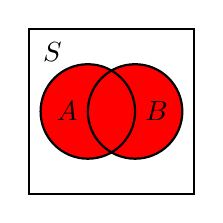
\begin{tikzpicture}[thick, scale=0.3]
  \draw (-3.5, -3.5) rectangle (3.5, 3.5);
  \filldraw[fill=red] (-1,0) circle [radius=2cm]
               (1,0) circle [radius=2cm];
  \draw (-1,0) node[left] {$A$};
  \draw (1,0) node[right] {$B$};
  \draw (-2.5,2.5) node {$S$};
\end{tikzpicture}
\end{center}
\end{frame}

\begin{frame}
\begin{Exercise}
  下列命题中哪个是真的?

A. 对任意集合$A$,$B$,$2^{A\cup B} = 2^A \cup 2^B$。

B. 对任意集合$A$,$B$,$2^{A\cap B} = 2^A \cap 2^B$。

C. 对任意集合$A$,$B$,$2^{A\setminus B} = 2^A \setminus 2^B$。

D. 对任意集合$A$,$B$,$2^{A\bigtriangleup B} = 2^A \bigtriangleup 2^B$。

\end{Exercise}
\pause
A.假
\begin{center}
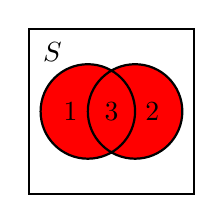
\begin{tikzpicture}[thick, scale=0.3]
  \draw (-3.5, -3.5) rectangle (3.5, 3.5);
  \filldraw[fill=red] (-1,0) circle [radius=2cm]
               (1,0) circle [radius=2cm];
  \draw (-1,0) node[left] {$1$};
  \draw (1,0) node[right] {$2$};
  \draw (0,0) node {$3$};
  \draw (-2.5,2.5) node {$S$};
\end{tikzpicture}
\end{center}
\end{frame}

\begin{frame}
\begin{Exercise}
  下列命题中哪个是真的?

A. 对任意集合$A$,$B$,$2^{A\cup B} = 2^A \cup 2^B$。

B. 对任意集合$A$,$B$,$2^{A\cap B} = 2^A \cap 2^B$。

C. 对任意集合$A$,$B$,$2^{A\setminus B} = 2^A \setminus 2^B$。

D. 对任意集合$A$,$B$,$2^{A\bigtriangleup B} = 2^A \bigtriangleup 2^B$。

\end{Exercise}
\pause
A.假

该结论不正确,这是因为设$A=\{1,3\},B=\{2,3\}$,则$\{1,2,3\}\in 2^{A\cup B}$,但是$\{1,2,3\}\notin 2^{A}\cup 2^{B}$。
\end{frame}

\begin{frame}
\begin{Exercise}
  下列命题中哪个是真的?

A. 对任意集合$A$,$B$,$2^{A\cup B} = 2^A \cup 2^B$。

B. 对任意集合$A$,$B$,$2^{A\cap B} = 2^A \cap 2^B$。

C. 对任意集合$A$,$B$,$2^{A\setminus B} = 2^A \setminus 2^B$。

D. 对任意集合$A$,$B$,$2^{A\bigtriangleup B} = 2^A \bigtriangleup 2^B$。

\end{Exercise}
\pause
A.假

该结论不正确,这是因为设$A=\{1\},B=\{2\}$,则$\{1,2\}\in 2^{A\cup B}$,但是$\{1,2\}\notin 2^{A}\cup 2^{B}$。
\end{frame}

\begin{frame}
\begin{Exercise}
  下列命题中哪个是真的?

A. 对任意集合$A$,$B$,$2^{A\cup B} = 2^A \cup 2^B$。


B. 对任意集合$A$,$B$,$2^{A\cap B} = 2^A \cap 2^B$。

C. 对任意集合$A$,$B$,$2^{A\setminus B} = 2^A \setminus 2^B$。

D. 对任意集合$A$,$B$,$2^{A\bigtriangleup B} = 2^A \bigtriangleup 2^B$。

\end{Exercise}
\pause
B.真
\pause
  \begin{equation*}
    \begin{split}
      \forall x \;&x \in 2^{A\cap B}\\
    \Leftrightarrow&x \subseteq A \cap B\\      
    \Leftrightarrow&\forall y\; y \in x \to y \in A \cap B\\
    \Leftrightarrow&\forall y\; y \in x \to y \in A \land y \in B\\
    \Leftrightarrow&(\forall y\; y \in x \to y \in A) \land (\forall y\; y \in x \to y \in B)\\
    \Leftrightarrow&x \subseteq A \land x \subseteq B\\
    \Leftrightarrow&x \in 2^A \land x \in 2^B\\
    \Leftrightarrow&x \in 2^A \cap 2^B\\    
    \end{split}
  \end{equation*}

\end{frame}
\begin{frame}
\begin{Exercise}
  下列命题中哪个是真的?

A. 对任意集合$A$,$B$,$2^{A\cup B} = 2^A \cup 2^B$。

B. 对任意集合$A$,$B$,$2^{A\cap B} = 2^A \cap 2^B$。

C. 对任意集合$A$,$B$,$2^{A\setminus B} = 2^A \setminus 2^B$。

D. 对任意集合$A$,$B$,$2^{A\bigtriangleup B} = 2^A \bigtriangleup 2^B$。

\end{Exercise}
\pause
C.假

该结论不成立,这是因为对任意集合$A$,$B$,$\phi \in 2^{A\setminus B}$,但是 $\phi \notin 2^A \setminus 2^B$。

\end{frame}
\begin{frame}
\begin{Exercise}
  下列命题中哪个是真的?

A. 对任意集合$A$,$B$,$2^{A\cup B} = 2^A \cup 2^B$。

B. 对任意集合$A$,$B$,$2^{A\cap B} = 2^A \cap 2^B$。

C. 对任意集合$A$,$B$,$2^{A\setminus B} = 2^A \setminus 2^B$。

D. 对任意集合$A$,$B$,$2^{A\bigtriangleup B} = 2^A \bigtriangleup 2^B$。

\end{Exercise}
\pause
D.假

该结论不成立,这是因为对任意集合$A$,$B$,$\phi \in 2^{A\bigtriangleup B}$,但是 $\phi \notin 2^A \bigtriangleup 2^B$。


\end{frame}

\begin{frame}
\begin{Exercise}
  下列命题中哪个是真的?

A. 对任意集合$A$,$B$,$2^{A\cup B} = 2^A \cup 2^B$。

B. 对任意集合$A$,$B$,$2^{A\cap B} = 2^A \cap 2^B$。

C. 对任意集合$A$,$B$,$2^{A\setminus B} = 2^A \setminus 2^B$。

D. 对任意集合$A$,$B$,$2^{A\bigtriangleup B} = 2^A \bigtriangleup 2^B$。

\end{Exercise}
\pause
\begin{minipage}{0.69\linewidth}
  \begin{Def}
    设$A,B$为任意的两个集合,$A\setminus B$与$B\setminus A$的并集称为$A$与$B$的对称差,记为$A \bigtriangleup B$。
    \begin{equation*}
      A\bigtriangleup B = (A \setminus B) \cup (B \setminus A)
    \end{equation*}
  \end{Def}
\end{minipage}
\begin{minipage}{0.29\linewidth}
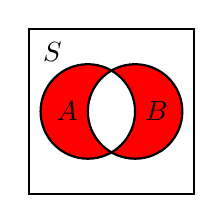
\begin{tikzpicture}[thick, scale=0.3]
  \draw (-3.5, -3.5) rectangle (3.5, 3.5);
\fill[red] (0,0 |- 60:2cm) arc [start angle=60, end angle = 300, radius = 2cm]
                           arc [start angle=240, end angle = 120, radius = 2cm];
\fill[red] (0,0 |- 60:2cm) arc [start angle=120, end angle = -120, radius = 2cm]
                           arc [start angle=-60, end angle = 60, radius = 2cm];
  \draw (-1,0) circle [radius=2cm]
               (1,0) circle [radius=2cm];
  \draw (-1,0) node[left] {$A$};
  \draw (1,0) node[right] {$B$};
  \draw (-2.5,2.5) node {$S$};
\end{tikzpicture}
\end{minipage}

设$A=\{1,2\}, B = \{1\}$,则

$2^{A\bigtriangleup B}=2^{\{2\}}=\{\phi, \{2\}\}$

$2^A \bigtriangleup 2^B=\{\phi, \{1\},\{2\},\{1,2\}\}\bigtriangleup\{\phi, \{1\}\} = \{\{2\},\{1,2\}\}$

$2^{A\bigtriangleup B} \ne 2^A \bigtriangleup 2^B$
\end{frame}


\end{CJK*}
\end{document}
